\documentclass[tikz, landscape, border=0]{standalone}

\usepackage{newpxtext}
\usepackage{newpxmath}
\usepackage{fontspec}
\usepackage{hyperref}  
 \usepackage[utf8]{inputenc}  
\catcode`\|12
% -----------------------------
\usetikzlibrary{calc}
\usetikzlibrary{intersections}
% -----------------------------
\usepackage{comandi}
% -----------------------------
\usetikzlibrary{decorations.markings}
\usetikzlibrary {decorations.text}
\usetikzlibrary { decorations.pathmorphing, decorations.pathreplacing, decorations.shapes}
\usetikzlibrary{matrix}
\usetikzlibrary {quotes} 
 \usepackage{pgf}

\newcommand{\titolo}{Comportamenti}
 
 % Definisci una macro per il testo
\newcommand{\primoComportamento}{
Questo gesto richiede una partenza lenta, in cui i microeventi sono intervallati da respiri. La parte concava della campana poggia sul palmo, che funge da coperchio. I parametri che possono influenzare il comportamento del gesto includono la continuità dell'azione, il punto in cui avviene la frizione (se più centrale o più esterno), e il movimento di apertura e chiusura del palmo rispetto al corpo della campana (il risultato sonoro consiste nella variazione del rumore intonato emesso dalla risonanza della campana).}

\newcommand{\secondoComportamento}{
Il gesto è da intendersi come conclusivo di un discorso iniziato con il gesto precedente, cercando di presentarlo in sincope rispetto a una pulsazione utilizzata per scandire alcuni accenti del gesto precedente. Deve essere sicuro ed è seguito da un respiro.}

\newcommand{\terzoComportamento}{
\' E una variazione sostanziale del primo gesto. permette il movimento all'interno e all'esterno con il battente sfregato lateralmente, e lungo la circonferenza con la parte inferiore del battente. \' E necessario cambiare il verso della rotazione in maniera inaspettata. Necessità una sempre maggiore articolazione dei comportamenti. }

\newcommand{\quartoComportamento}{Il flusso complessivo è simile a quello di un circuito di un filtro, in cui alcuni rami di \textit{feedback} presentano frecce orientate in senso opposto rispetto al flusso temporale del brano.

I percorsi segnati da linee più spesse vanno attraversati un maggior numero di volte, variando progressivamente il gesto e simulando il meccanismo di feedback.

I rami che ruotano attorno ai gesti sono anch'essi dei rami di feedback.}





\begin{document}
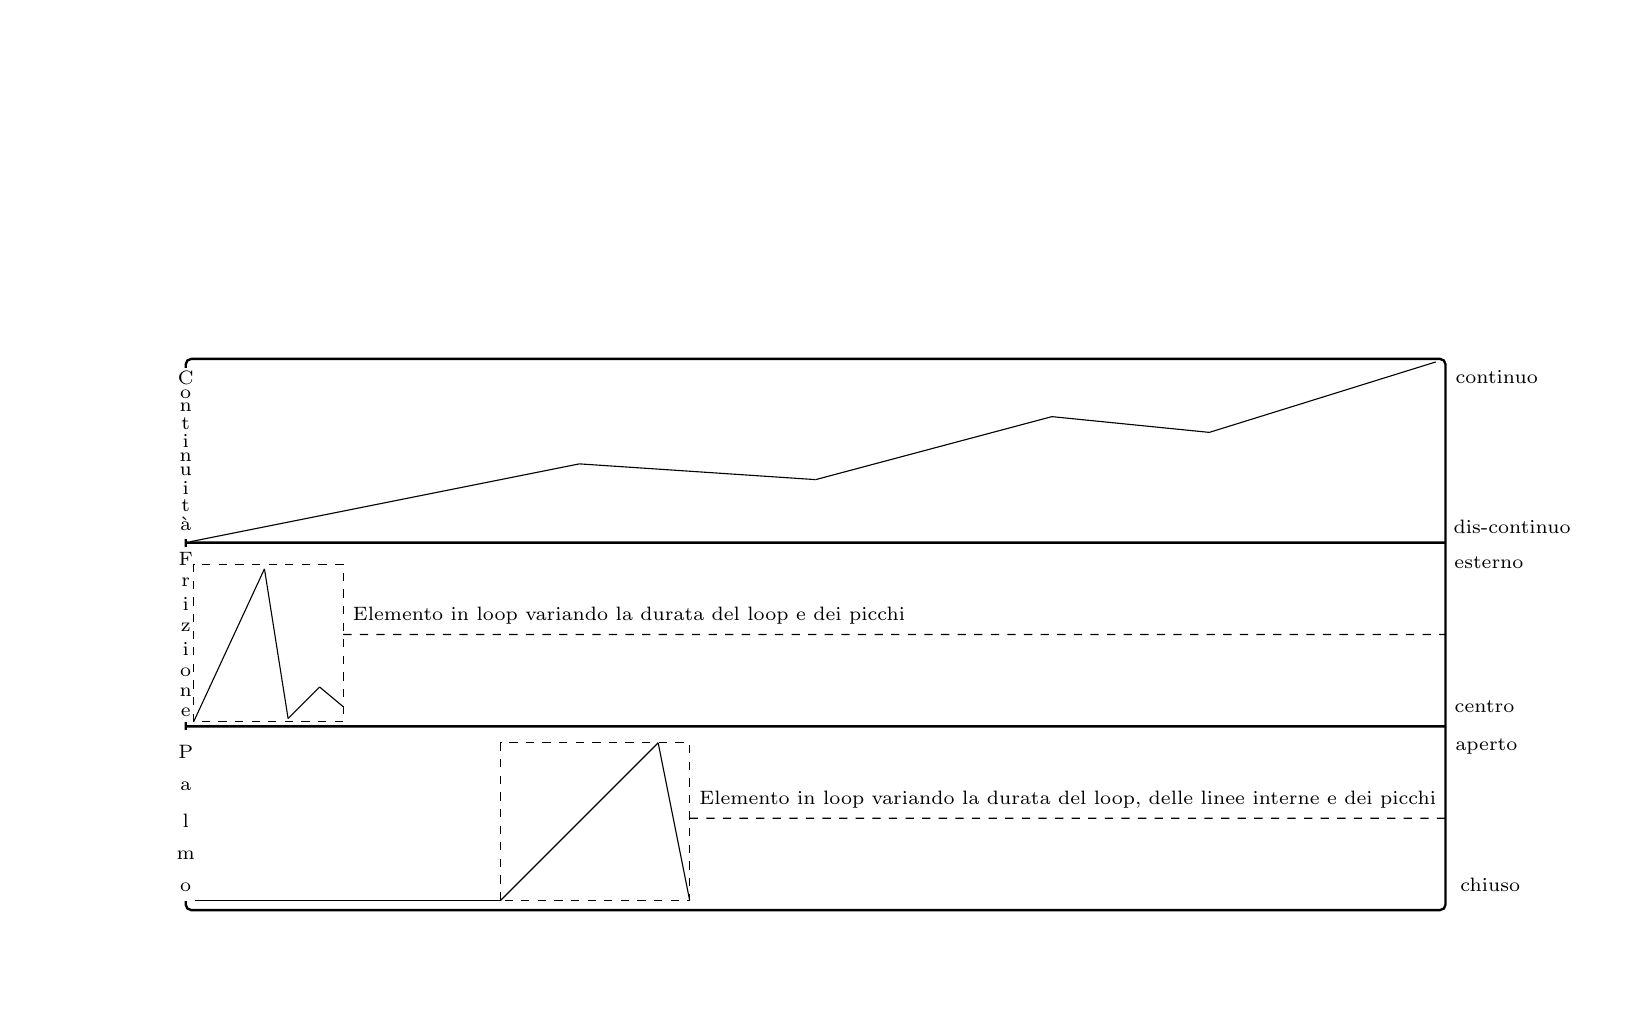
\begin{tikzpicture}[every edge quotes/.style={fill=white,font=\footnotesize}]


%======================================================================
% ------------------------------ preparazione foglio di lavoro ----------------------------------------------------
\def\RealpaperHeight{29.7cm}
\def\RealpaperWidth{42cm}
\def\zeroX{1cm}
\def\zeroY{2.5cm}
\def\paperHeight{\RealpaperHeight-\zeroY}
\def\paperWidth{\RealpaperWidth-\zeroX}

%\draw[step=.01cm, gray, line width = 0.01pt] (0, 0) grid (\paperWidth, \paperHeight); 
%\draw[step=.1cm, gray, very thin] (0, 0) grid (\paperWidth, \paperHeight); 
%\draw[step=.5cm, gray, ultra thin] (0, 0) grid (\RealpaperWidth, \RealpaperHeight);
%\draw[step=1cm, black, very thin] (0, 0) grid (\paperWidth, \paperHeight); 
%\draw[black, very thick, dotted] (\RealpaperWidth/2,\zeroY) -- (\RealpaperWidth/2,\paperHeight);
%\draw[black, very thick, dotted] (\zeroX,\RealpaperHeight/2) -- (\paperWidth,\RealpaperHeight/2);
%\draw (\zeroX,\zeroY) rectangle (\paperWidth,\paperHeight);

%======================================================================



%======================================================================
% Posizionamento delle carte in cerchio
\def\circleRadius{11cm}  % Regola questo valore in base alle tue esigenze
\def\numCards{11}  % Numero di carte nel cerchio principale
\def\angleOffset{30}  % Offset angolare per ruotare l'intero layout
% ------------------
\def\pointWidth{3pt}
% ------------------
\def\minimumSize{1.5pt}
% ------------------
\def\arrowWidth{6pt}
\def\arrowLength{9pt}
\def\sumWidth{1pt}
\def\lineWidthMore{3pt}
\def\lineWidthMedium{\lineWidthMore-1.5}
\def\lineWidth{\lineWidthMore-2.5pt}
\def\arrowWidthMore{9pt}
\def\arrowLengthMore{12pt}
\def\sumWidthMore{3pt}
\def\roundedCorners{8pt}
% ------------------
\def\cardRadius{1.5cm} 
\def\cardRadiusTwo{\cardRadius + .5cm} 
% ------------------
\def\battenteheight{.25}
\def\battentewidth{1.3}
%======================================================================








%======================================================================
% ------------------------------  Nodo per il gesto nel rettangolo  -----------------------------------------------
%
\draw[opacity=0] ({\zeroX},{\paperHeight + \zeroY}) node[below right, yshift={0.435*\paperHeight},xshift={0.15*\paperHeight}] (firstRect) {} rectangle ++({0.5*\paperWidth },{0.5*\paperHeight })  node[pos=.1,yshift={-.085cm},name=LDuno] {}node[pos=.1,yshift={+6.915cm},name=LUuno] {} node[pos=.9,yshift={-9.965cm},name=RDuno] {}node[pos=.9,yshift={-2.965cm},name=RUuno] {};
%======================================================================


\draw[line width=.03cm,rounded corners=2pt] (LDuno.center) rectangle (RUuno.center) ;













%======================================================================
% -----------------------------	comportamento 1		-------------------------------------------------------
%
% create 2 points LEFT
\node[inner sep = 0pt, minimum size = .1cm, name = LUMuno] at ($(LUuno)!0.333333!(LDuno)$){};
\node[inner sep = 0pt, minimum size = .1cm,name=LDMuno] at ($(LUMuno)!0.5!(LDuno)$){};
% create 2 points RIGHT
\node[inner sep = 0pt, minimum size = .1cm, name = RUMuno] at ($(RUuno)!0.333333!(RDuno)$){};
\node[inner sep = 0pt, minimum size = .1cm, name = RDMuno] at ($(RUMuno)!0.5!(RDuno)$){};

% create a LINE SEP
\draw[line width=.03cm] (LUMuno.center) -- (RUMuno.center);
\draw[line width=.03cm] (LDMuno.center) -- (RDMuno.center);
% ---------------------
    % Definiamo una matrice per scrivere le lettere lungo la linea
    \draw[fill,white] (LUuno.south west) rectangle (LUMuno.north east);
    \matrix[matrix of nodes,
            nodes={anchor=center,fill=white,},
            column sep=0pt, row sep=.07cm] 
            at ($(LUuno)!0.5!(LUMuno)$)
                {
        |[inner sep=0pt]| \scriptsize C \\ 
        |[inner sep=0pt]| \scriptsize o \\
        |[inner sep=0pt]| \scriptsize n \\
        |[inner sep=0pt]| \scriptsize t \\
        |[inner sep=0pt]| \scriptsize i \\
        |[inner sep=0pt]| \scriptsize n \\ 
        |[inner sep=0pt]| \scriptsize u \\
        |[inner sep=0pt]| \scriptsize i \\
        |[inner sep=0pt]| \scriptsize t \\
        |[inner sep=0pt]| \scriptsize à \\
    };
\node[circle, xshift=-.15cm,yshift=-.1cm, right] at (RUuno.south east) {\scriptsize continuo};
\node[circle, xshift=-.10cm,yshift=.15cm, right] at (RUMuno.north east) {\scriptsize dis-continuo};
% ---------------------
    % Definiamo una matrice per scrivere le lettere lungo la linea
    \draw[fill,white] (LUMuno.south west) rectangle (LDMuno.north east);
    \matrix[matrix of nodes,
            nodes={anchor=center,fill=white,},
            column sep=0pt, row sep=.15cm] 
            at ($(LUMuno)!0.5!(LDMuno)$)
                {
        |[inner sep=0pt]| \scriptsize F \\ 
        |[inner sep=0pt]| \scriptsize r \\
        |[inner sep=0pt]| \scriptsize i \\
        |[inner sep=0pt]| \scriptsize z \\
        |[inner sep=0pt]| \scriptsize i \\
        |[inner sep=0pt]| \scriptsize o \\ 
        |[inner sep=0pt]| \scriptsize n \\
        |[inner sep=0pt]| \scriptsize e \\
    };
\node[circle, xshift=-.1cm,yshift=-.2cm,right] at (RUMuno.south east) {\scriptsize esterno};
\node[circle, xshift=-.1cm,yshift=.2cm,right] at (RDMuno.north east) {\scriptsize centro};
% ---------------------
    % Definiamo una matrice per scrivere le lettere lungo la linea
    \draw[fill,white] (LDMuno.south west) rectangle (LDuno.north east);
    \matrix[matrix of nodes,
            nodes={anchor=center,fill=white,},
            column sep=0pt, row sep=.3cm] 
            at ($(LDMuno)!0.5!(LDuno)$)
                {
        |[inner sep=0pt]| \scriptsize P \\ 
        |[inner sep=0pt]| \scriptsize a \\
        |[inner sep=0pt]| \scriptsize l \\
        |[inner sep=0pt]| \scriptsize m \\
        |[inner sep=0pt]| \scriptsize o \\
    };


\node[circle, xshift=-.1cm,yshift=-.2cm,right] at (RDMuno.south east) {\scriptsize aperto};
\node[circle, xshift=-.1cm,yshift=.2cm,right] at (RDuno.north east) {\scriptsize chiuso};
% ---------------------    
% linea continuità
\node (fineuno) at (RUuno){};
%\draw (LUMuno) -- (fineuno);
\draw (LUMuno) -- ($(LUMuno)+(5,1)$);
\draw ($(LUMuno)+(5,1)$) -- ($(LUMuno)+(8,.8)$);
\draw ($(LUMuno)+(8,.8)$) -- ($(LUMuno)+(11,1.6)$);
\draw ($(LUMuno)+(11,1.6)$) -- ($(LUMuno)+(13,1.4)$);
\draw ($(LUMuno)+(13,1.4)$) -- (fineuno);
    

\node (fineuno) at (RUMuno){};
%\draw (LDMuno) -- (fineuno);
\draw ($(LDMuno.north)+(.1,0)$) -- ($(LDMuno)+(1,2)$);
\draw ($(LDMuno)+(1,2)$) -- ($(LDMuno)+(1.3,.1)$);
\draw ($(LDMuno)+(1.3,.1)$) -- ($(LDMuno)+(1.7,.5)$);
\draw ($(LDMuno)+(1.7,.5)$) -- ($(LDMuno)+(2,.25)$);
\draw[dashed] ($(LDMuno.north)+(.1,0)$) rectangle ($(LDMuno.north)+(2,2)$);
\node (fine) at ($(LDMuno)+(2,0)$) {};
\node (fineDue) at ($(LUMuno)+(2,0)$) {};
\node[above right] (robbba) at ($(fine)!0.5!(fineDue)$) {\scriptsize Elemento in loop variando la durata del loop e dei picchi};
\draw[dashed] ($(fine)!0.5!(fineDue)$) -- ($(RUMuno)!0.5!(RDMuno)$);

\node (fineuno) at (RDMuno){};
%\draw (LDuno) -- (fineuno);
\draw (LDuno.north east) -- ($(LDuno.north)+(4,0)$);
\draw  ($(LDuno.north)+(4,0)$) --($(LDuno.north)+(6,2)$);
\draw  ($(LDuno.north)+(6,2)$) --($(LDuno.north)+(6.4,0)$);
\draw[dashed] ($(LDuno.north)+(4,0)$) rectangle ($(LDuno.north)+(6.4,2)$);
\node (fine) at ($(LDuno)+(6.4,0)$) {};
\node (fineDue) at ($(LDMuno)+(6.4,0)$) {};
\node[above right] (robbba) at ($(fine)!0.5!(fineDue)$) {\scriptsize Elemento in loop variando la durata del loop, delle linee interne e dei picchi};
\draw[dashed] ($(fine)!0.5!(fineDue)$) -- ($(RDuno)!0.5!(RDMuno)$);
%=====================================================================


\end{tikzpicture}
\end{document}